\documentclass[]{jarticle}          % 一段組
%\documentclass[twocolumn]{jarticle} % 二段組

\textwidth 180mm
\textheight 255mm
\oddsidemargin -12mm
\topmargin -15mm
\columnsep 10mm

%\vspace{0.5cm} % 一段組の場合はコメントアウトした方が体裁がよいx
%] % 一段組の場合はコメントアウトする

\usepackage{styles/labheadings}
\usepackage[dvipdfmx]{graphicx,color}
\usepackage{amsmath,amssymb}
\usepackage{url}
% 追加
\usepackage[hang,small,bf]{caption}
\usepackage[subrefformat=parens]{subcaption}
\usepackage{float}
\captionsetup{compatibility=false}

\input{numerical_definition.tex}
% report.texと同じディレクトリにnumerical_definition.texを入れておけば上の書き方でもいいはずです

\usepackage[
  dvipdfm,
  bookmarks=true,
  bookmarksnumbered=true,
  colorlinks=true]{hyperref}
\AtBeginDvi{\special{pdf:tounicode EUC-UCS2}}

\pagestyle{labheadings}
\headerleft{全方位画像を用いたシーンの3次元モデルの作成とその活用}   % ヘッダの左側のタイトル
\headerright{2025年4月7日}  % ヘッダの右側のタイトル

\begin{document}

%\twocolumn % 一段組の場合はコメントアウトする

\vspace*{2ex}
\begin{center}
 {\Large \bf 研究の概要と1年間の進捗}\\ % タイトル
 \vspace*{5mm}
 {\large M2 田川幸汰}% 発表者名
\end{center}

%\vspace{0.5cm} % 一段組の場合はコメントアウトした方が体裁がよいx
%] % 一段組の場合はコメントアウトする

%新しく作成したコマンド
% \newcommand{\reffig}[1]{\hyperref[#1]{図\ref{#1}}}
% \newcommand{\refeq}[1]{\hyperref[#1]{式(\ref{#1})}}
% \newcommand{\reftab}[1]{\hyperref[#1]{表\ref{#1}}}
% \newcommand{\refsec}[1]{\hyperref[#1]{\ref{#1}章}}
% \newcommand{\refsubsec}[1]{\hyperref[#1]{\ref{#1}節}}

% 数式
%\begin{equation}
%  数式記述  
%  \label{ラベル名}
%\end{equation}

% 図
% \begin{figure}[!ht]
%   \begin{center}
%     \includegraphics[scale=0.5]{figures/画像ファイル名}
%     \caption{キャプション名}
%     \label{ラベル名}
%   \end{center}
% \end{figure}

% リスト
% \begin{enumerate or itemize}
%   \item 
% \end{enumerate or itemize}

\section{概要}
\subsection{研究背景}
近年、デジタルツインの市場規模が急速に拡大しており、現実空間の高精度なデジタル再現技術が多様な分野で求められている\cite{bib1}。
特に、屋内外の空間情報をリアルタイムに反映し、ナビゲーションや現場管理に活用するニーズが高まっている。
しかし、一般的な3次元モデルの構築では、多視点からの多数の画像撮影が必要となる上に、
テクスチャを滑らかに割り当てるには高度な撮影技術や、専門のソフト等が必要となる。
これらの問題はデジタルツインの現場導入を妨げる要因となっている\cite{bib2}。
\subsection{研究目的}
本研究では、全方位画像を活用して、簡易かつ効率的に高品質なテクスチャ付き3次元モデルを生成し、
それを用いた実用的な自己位置推定手法の確立を目指す。
全方位画像の活用により、多視点からの撮影や特別な撮影手段を必要とせず、簡易にデジタルツイン環境を構築することが可能となる。
さらに、本手法はセンサやGPSに依存しないため、専用機材を新たに導入する必要がなく、
屋内などセンサ情報の取得が困難な環境において、有効なテクスチャマッピング手法を提供できる。
また、現実空間を3次元モデルとして再現しながら自己位置推定を行うことで、
ナビゲーションや現場管理支援といった実用的なニーズに応える技術基盤を構築する。
\subsection{手法の概要}
\begin{enumerate}
  \item 全方位カメラのパラメータ推定
  \begin{itemize}
    \item 2次元座標と3次元座標の対応を用いて全方位カメラの位置と角度を推定する。
  \end{itemize}
  
  \item テクスチャの割り当て
  \begin{itemize}
    \item 全方位画像から取得したテクスチャと、
    建物の壁と床を単純な平面で表現した3次元ワイヤーフレームモデルを組み合わせてシーンを再現する。
  \end{itemize}
  
  \item ユーザ画像との自動対応付けによる自己位置推定
  \begin{itemize}
    \item 入力画像と3次元モデルの対応点を自動で抽出し、位置を推定する。
  \end{itemize}
\end{enumerate}
  
\section{全方位カメラのパラメータ推定}
全方位画像から任意視線方向の透視投影画像を生成し、透視投影画像上の2次元座標と3次元モデルの頂点を対応付ける。
カメラ位置姿勢の推定には、直交射影の共線性と共面性を用いた手法\cite{bib3}を用いる。
共線性とは、3次元点と画像面上の点が誤差なく対応する時、3次元点はカメラ中心から画像面上のベクトル上に存在することである。
また共面性とは、3次元直線と画像面上の直線が誤差なく対応する時、3次元直線はカメラ中心と画像面上の直線が構成する平面上に存在することである。
これらの誤差を最小化することで、カメラパラメータを推定する手法である。
\subsection{推定結果}
入力した全方位画像を図\ref{one}に示す。
\begin{figure}[H]
  \begin{center}
    \begin{tabular}{c}
      \includegraphics[width=0.8\textwidth]{figures/eimage_1.jpg}
    \end{tabular}
  \end{center}
  \caption{全方位画像}
  \label{one}
\end{figure}
パラメータ推定に用いた透視投影画像および2次元座標を図\ref{two}に示す。
\begin{figure}[H]
  \begin{center}
    \begin{tabular}{cc}
      \includegraphics[width=0.4\textwidth]{figures/cam0.png}
      \includegraphics[width=0.4\textwidth]{figures/cam1.png}\\
    \end{tabular}
  \end{center}
  \caption{透視投影画像}
  \label{two}
\end{figure}
パラメータの推定結果を表\ref{three}に示す。今回はカメラの位置を表す並進ベクトルのみ示す。
\begin{figure}[H]
  \begin{center}
    \begin{tabular}{lcc}
    & 推定結果(cm) & 実測値との誤差(cm) \\
    x & 100.45 & 0.45 \\
    y & 395.58 & -4.41 \\
    z & 136.82 & 1.82
    \end{tabular}
  \end{center}
  \caption{パラメータの推定結果}
  \label{three}
\end{figure}
実測値との精度比較では、いずれの条件においても誤差はおおむね10cm以内に収まることが多い。
\section{テクスチャの割り当て}
先ほど推定したカメラパラメータをもとに、テクスチャを割り当てる。
テクスチャを割り当てる際の工夫したポイントは以下の4点である。
\subsection{手法の概要}
\begin{enumerate}
  \item テクスチャ割り当ての条件
  \begin{itemize}
    \item 複数の全方位カメラで同一領域のテクスチャを取得する際、重心がカメラ中心に近いテクスチャを優先する。
  \end{itemize}
  
  \item テクスチャの明るさ調整
  \begin{itemize}
    \item 撮影環境による明るさの差を補正し、滑らかなシーンを再現する。
  \end{itemize}
  
  \item 側面部分のテクスチャ形状を四角形に変更
  \begin{itemize}
    \item 店舗の壁面や正面の直線的な形状に自然に合うように変更し、透視投影の際に発生する歪みを射影変換により解消する。
  \end{itemize}
\end{enumerate}

\subsection{生成したテクスチャ及び3次元モデル}
取得したテクスチャの一部を図\ref{four}に示す。
\begin{figure}[H]
  \begin{center}
    \begin{tabular}{cc}
      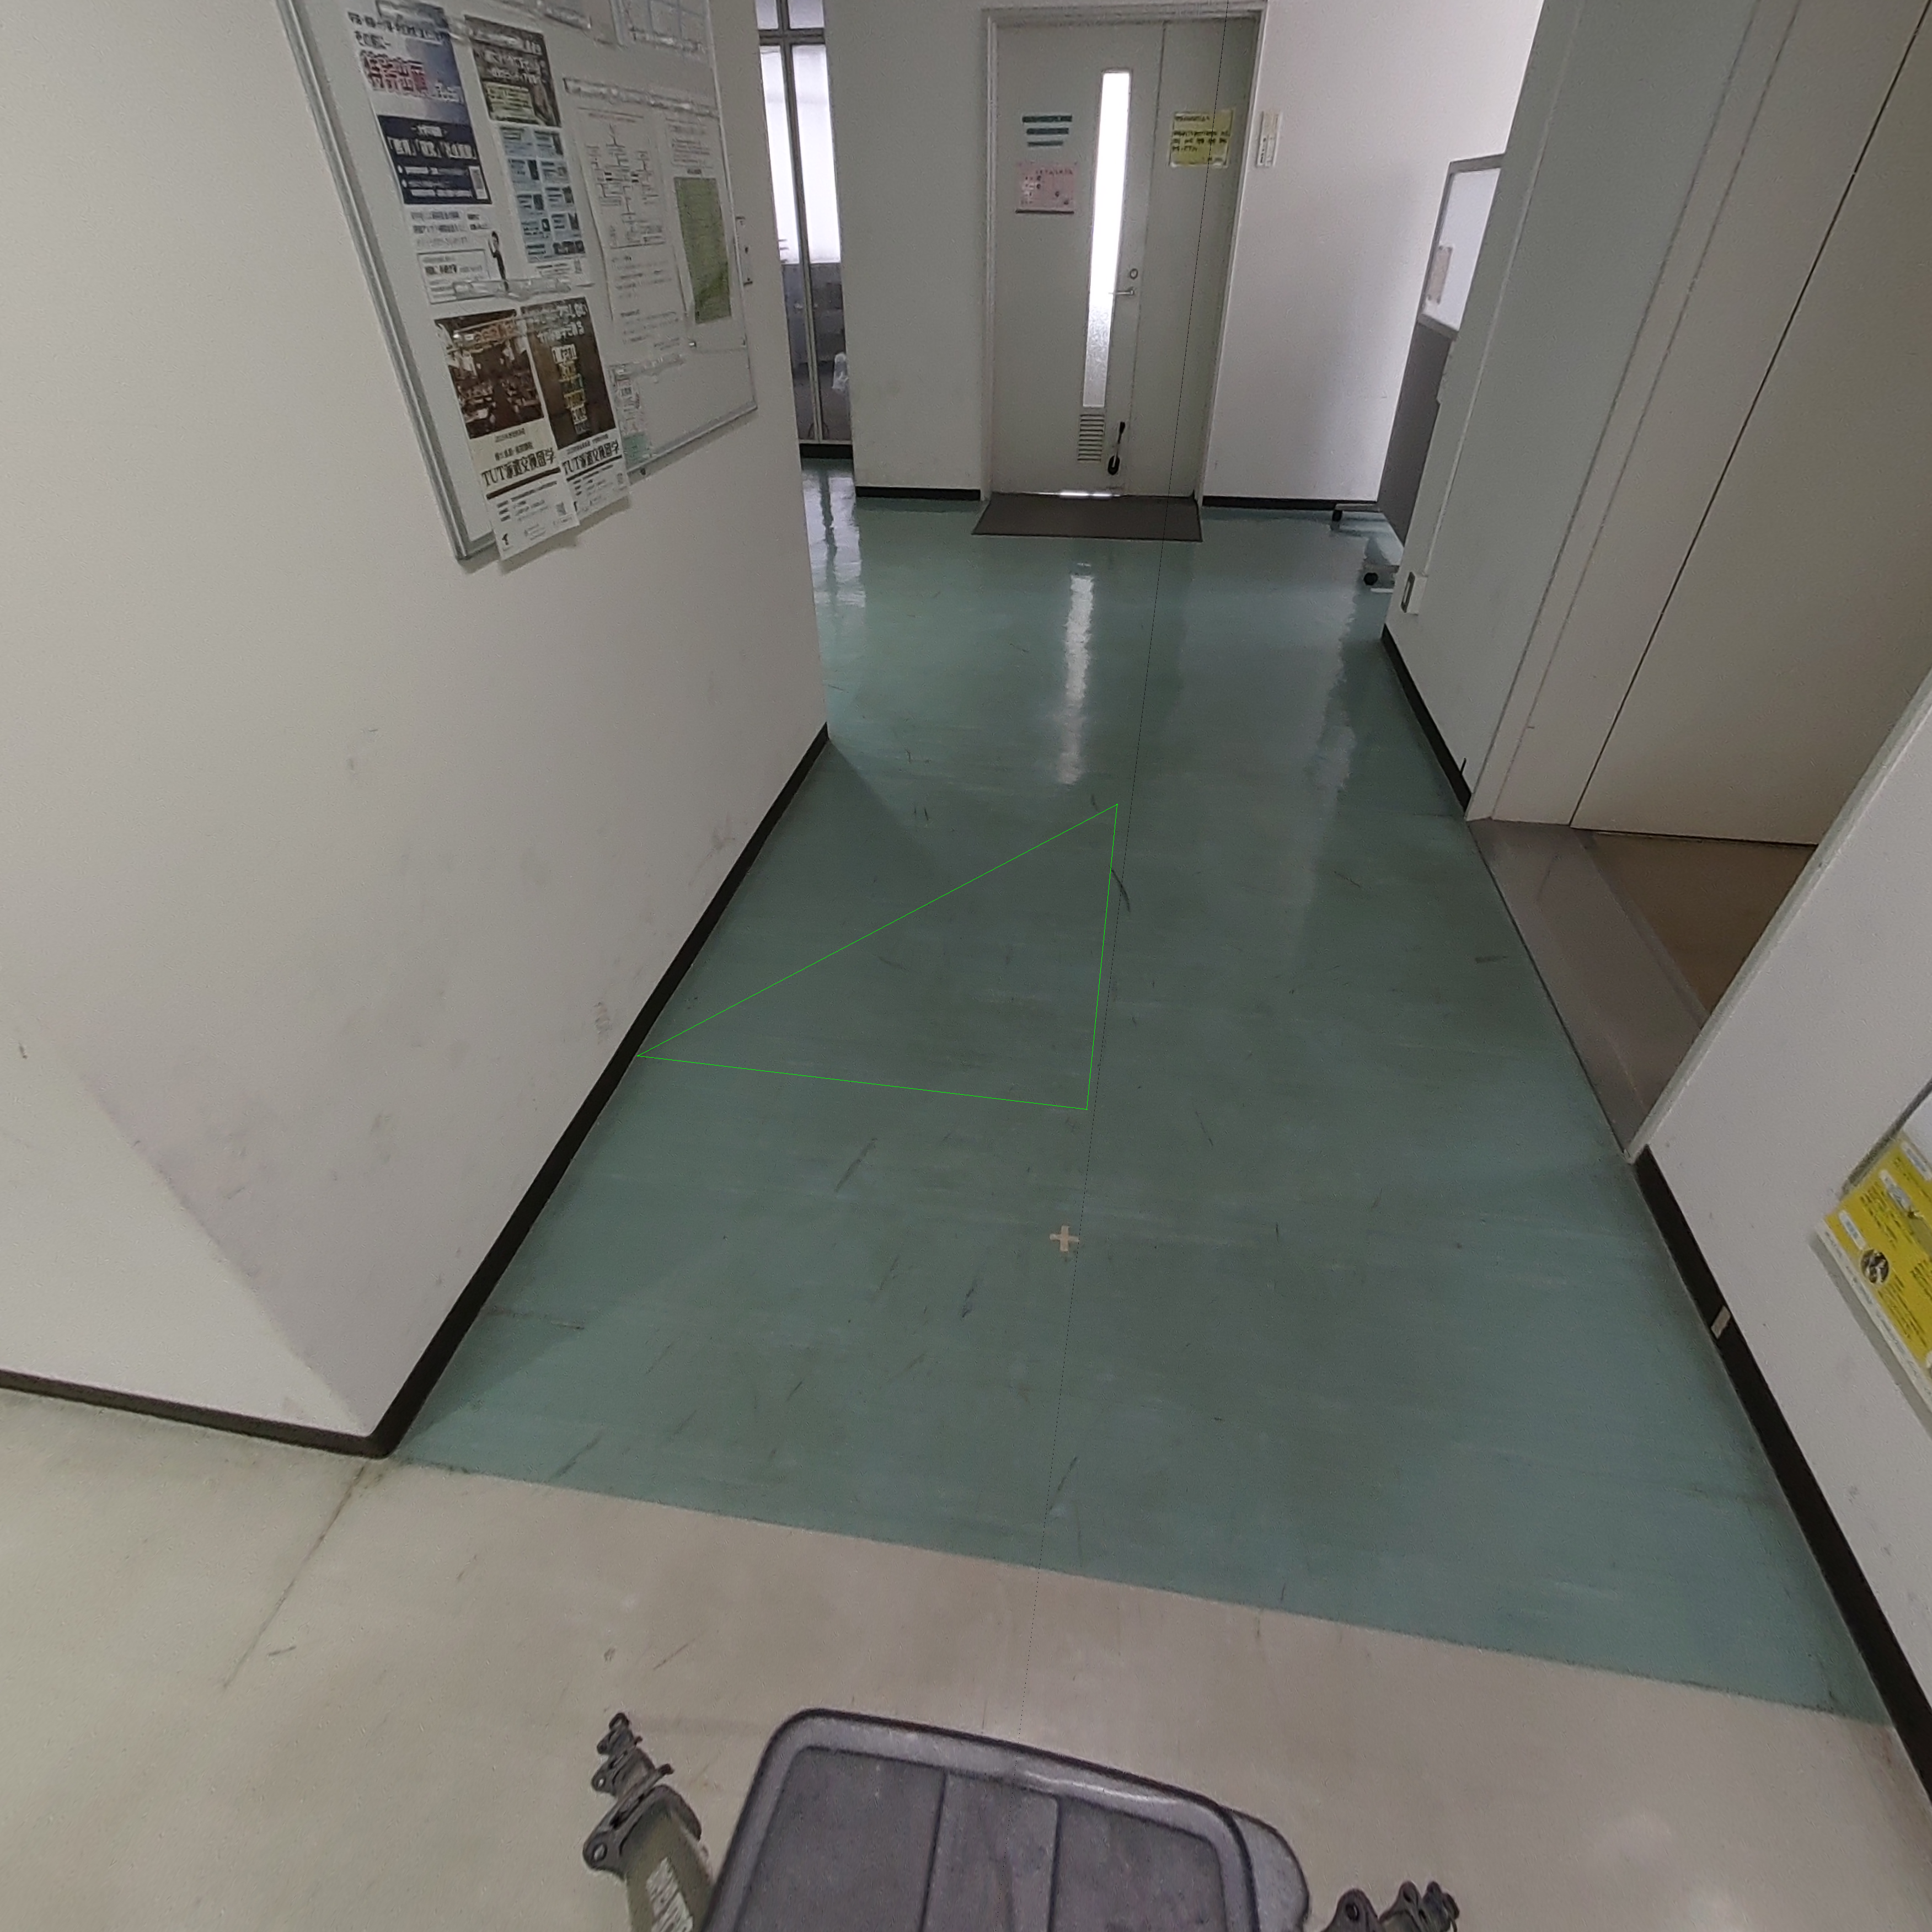
\includegraphics[width=0.4\textwidth]{figures/texture_1_6.png}&
      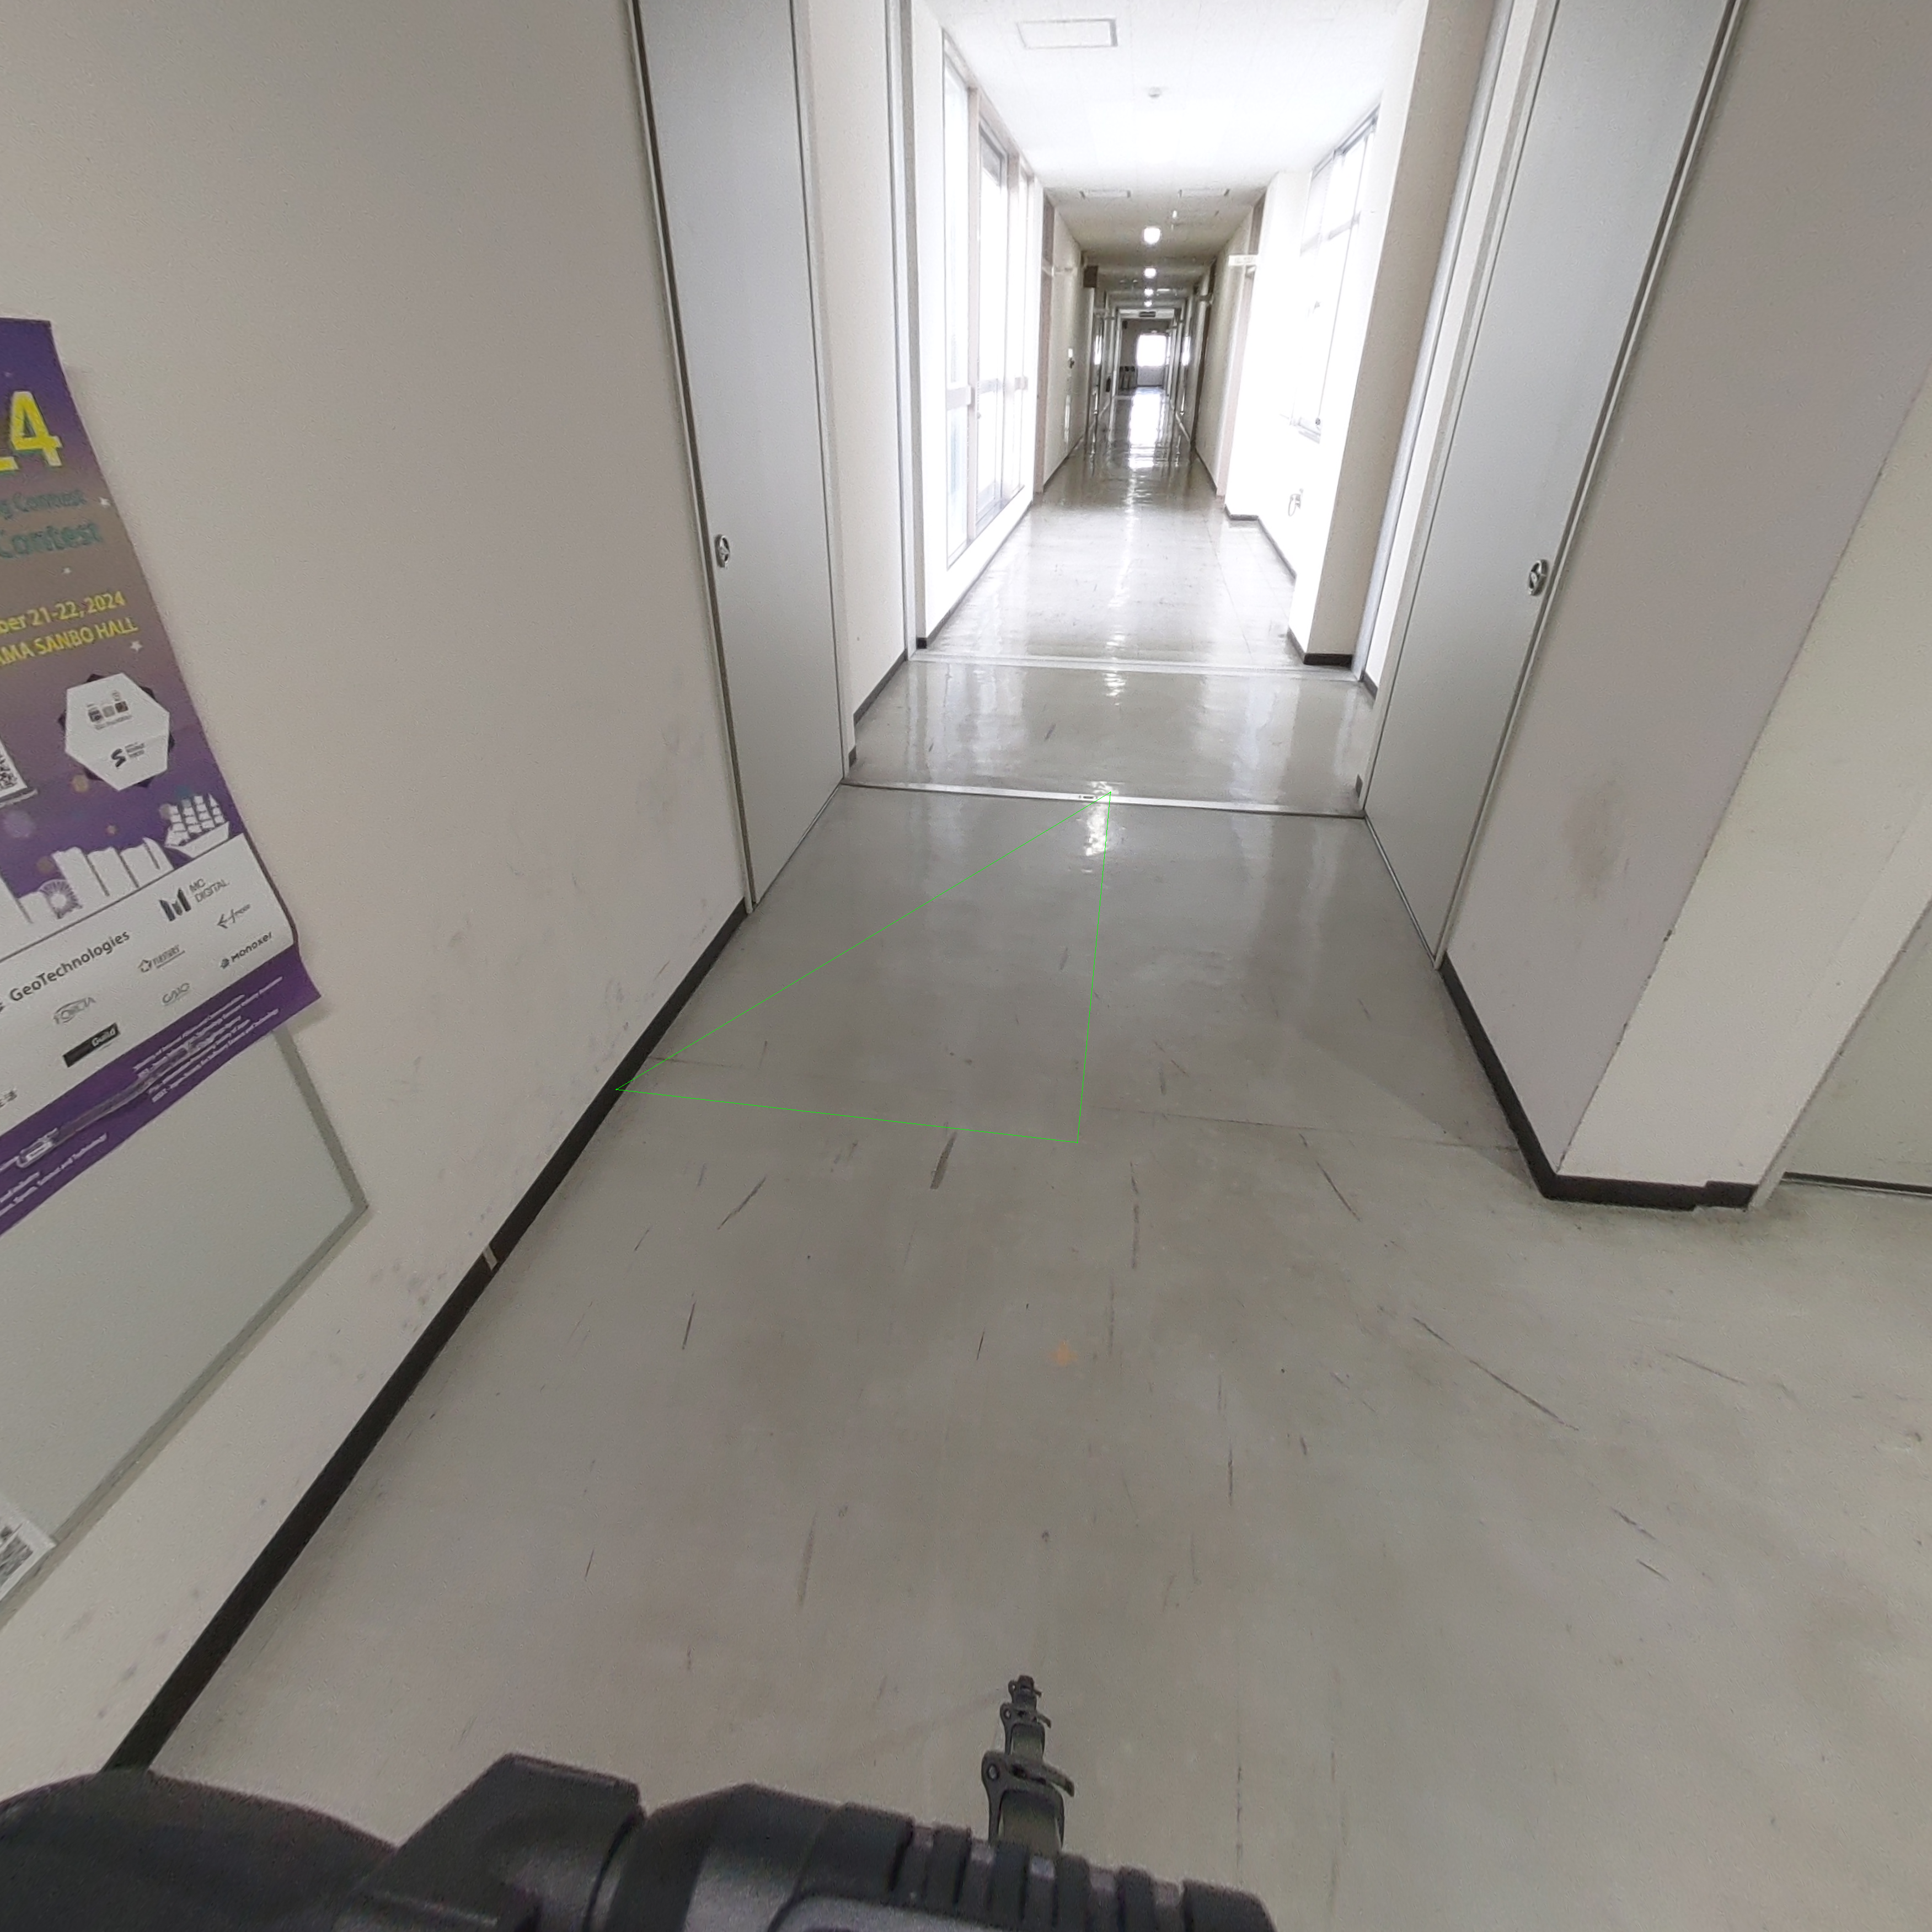
\includegraphics[width=0.4\textwidth]{figures/texture_1_19.png}\\
      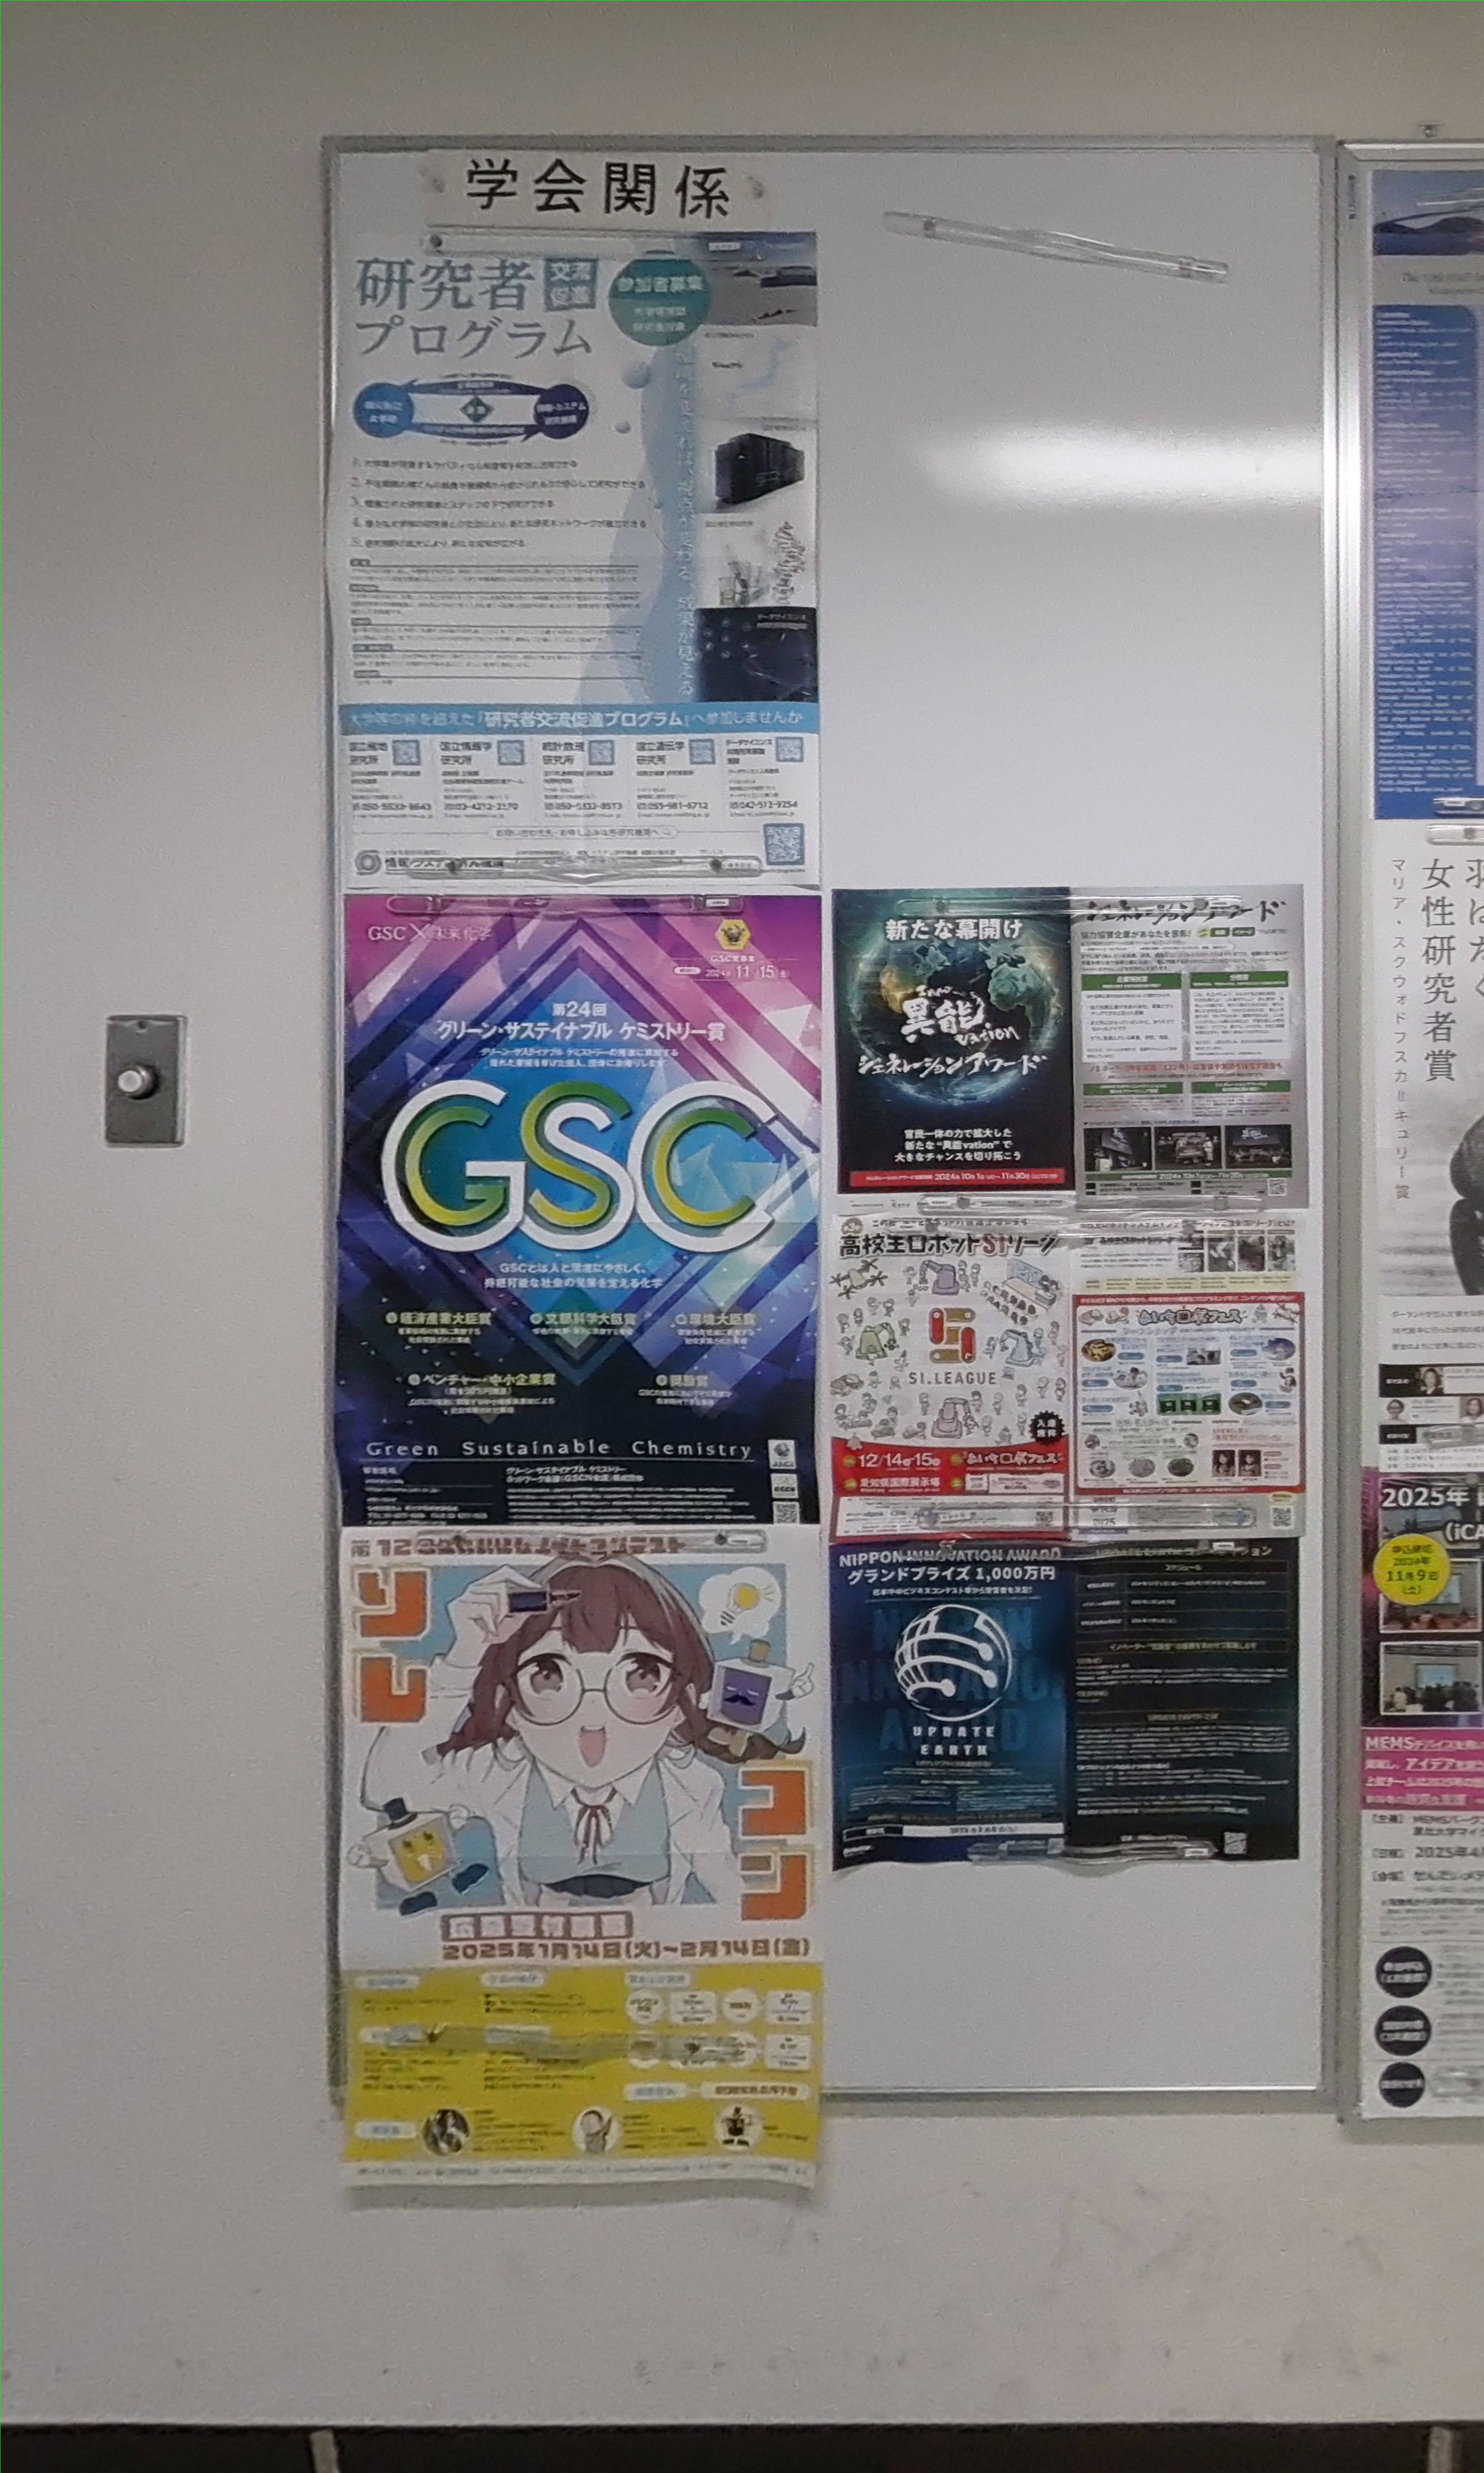
\includegraphics[width=0.4\textwidth]{figures/texture_1_46.png}&
      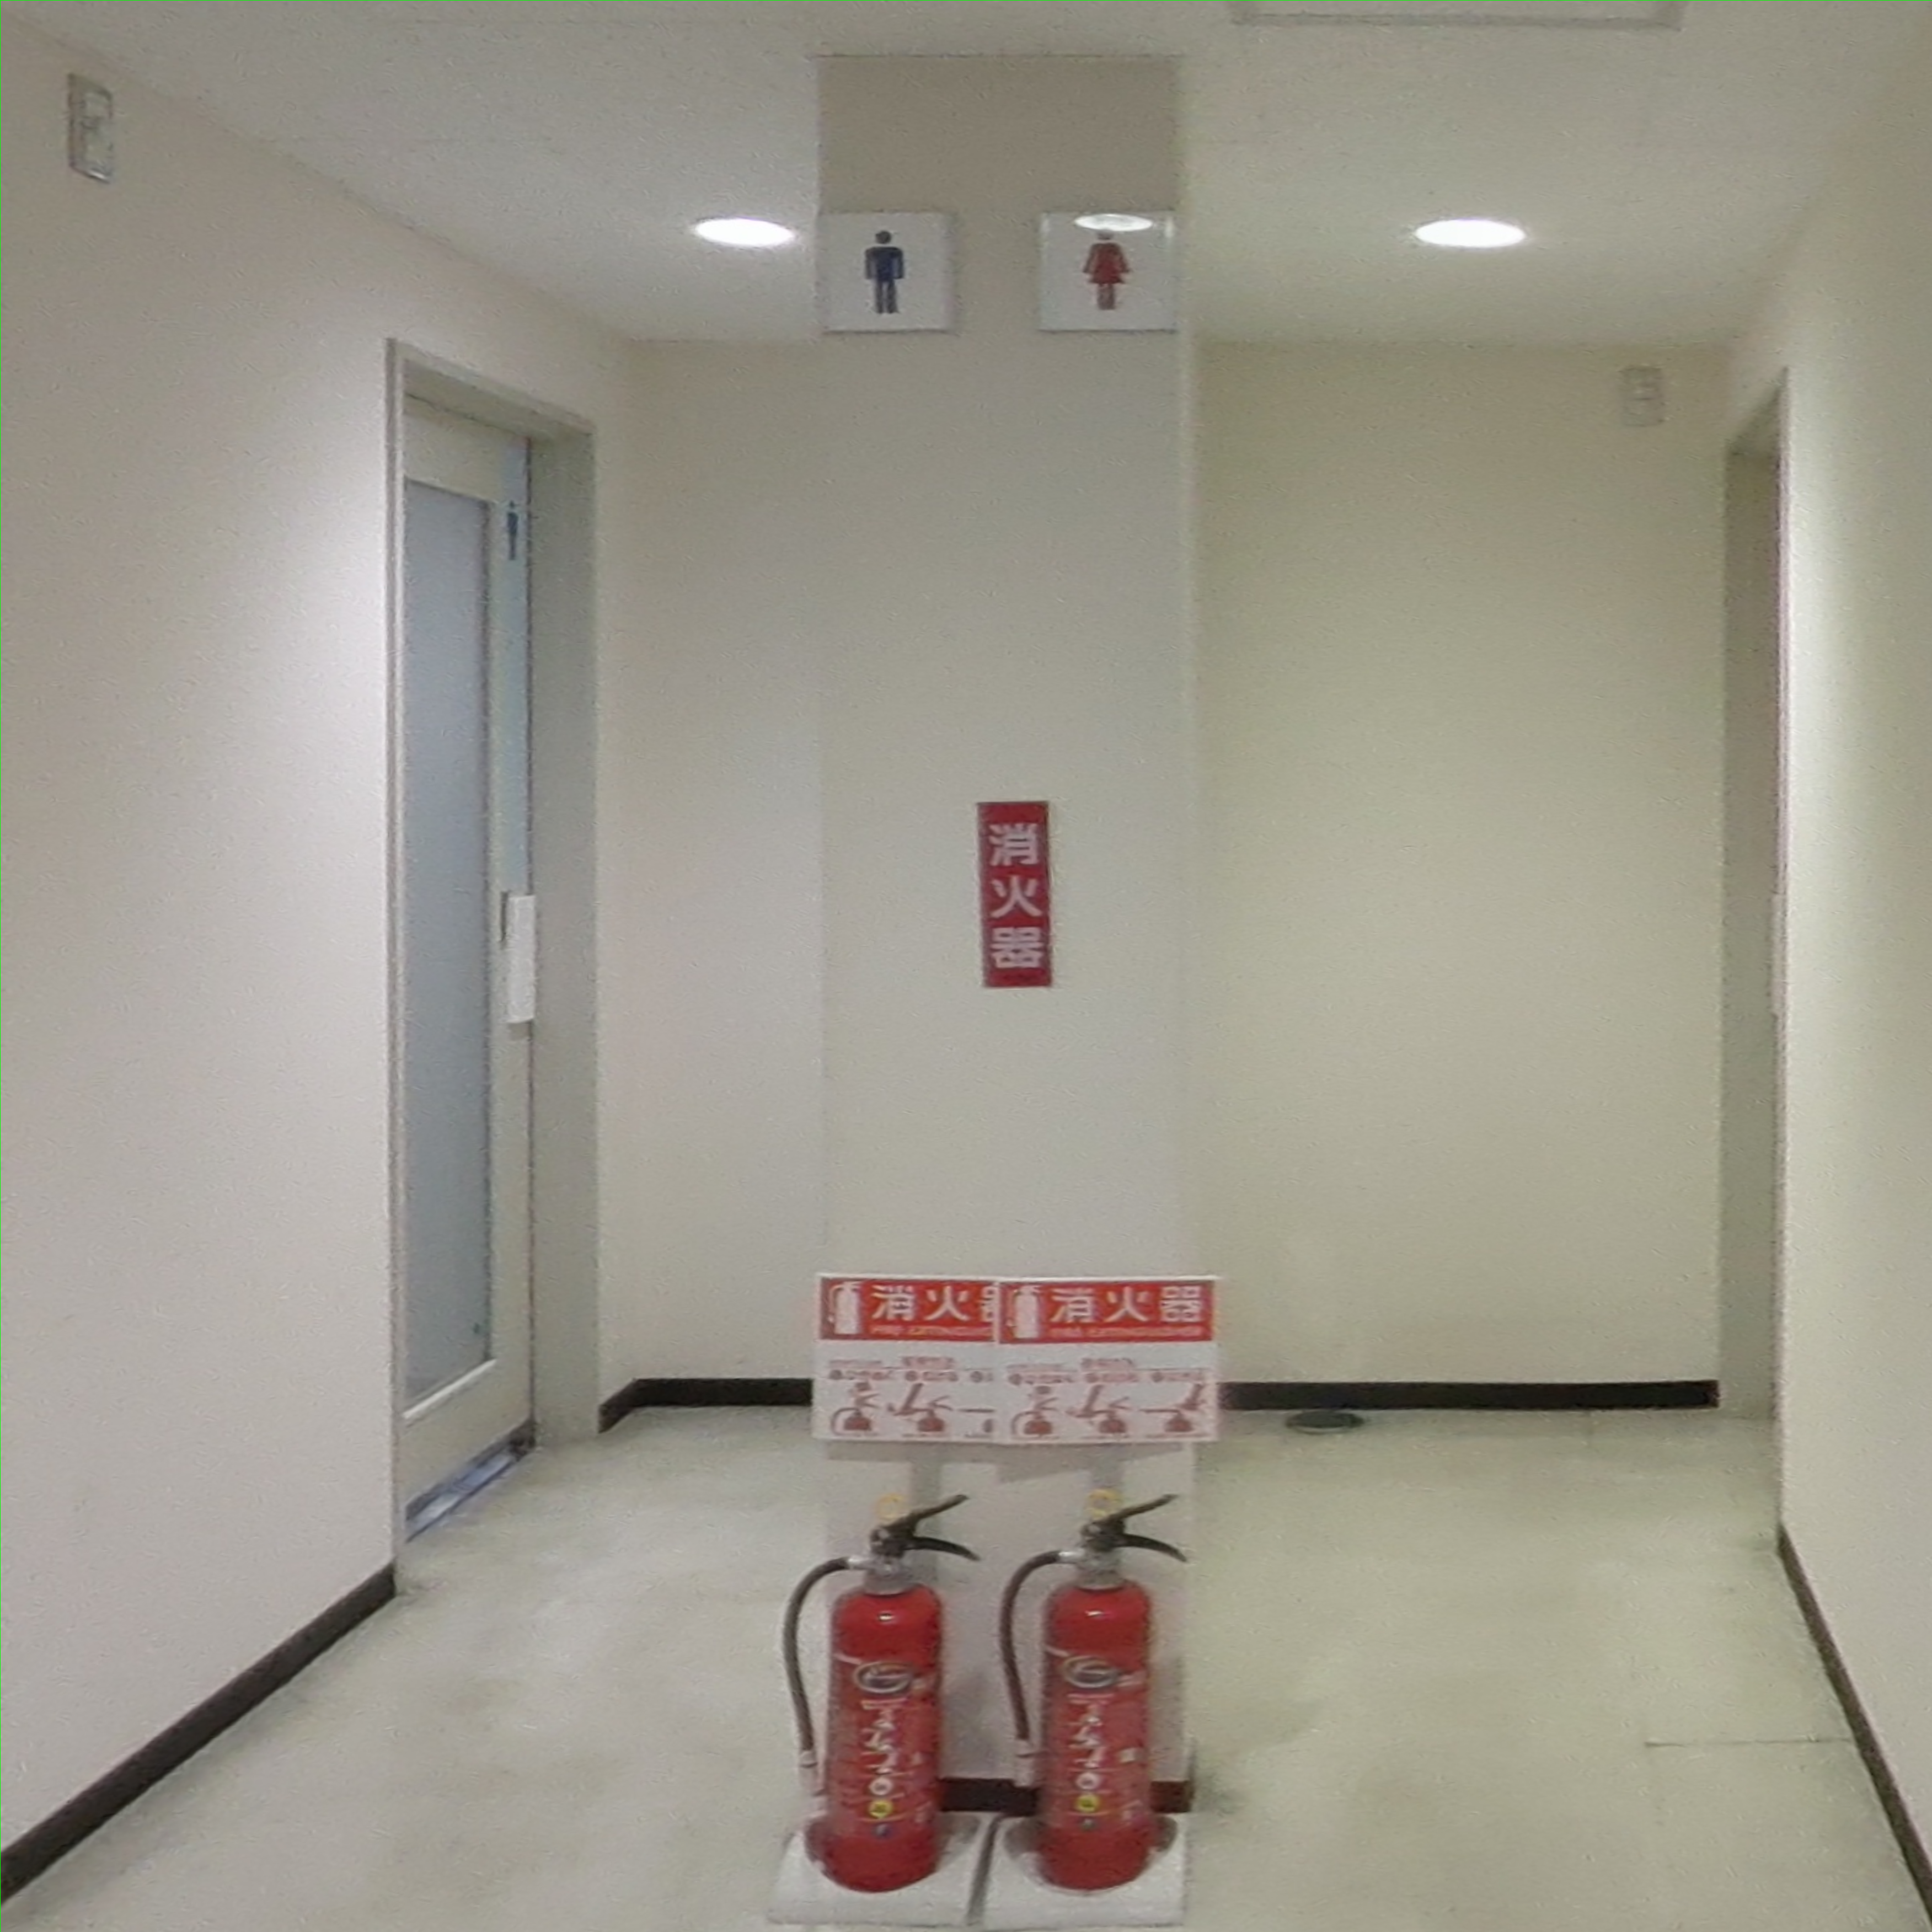
\includegraphics[width=0.4\textwidth]{figures/texture_1_52.png}\\
    \end{tabular}
  \end{center}
  \caption{テクスチャ画像}
  \label{four}
\end{figure}
テクスチャを割り当てた3次元モデルを図\ref{five}に示す。
\begin{figure}[H]
  \begin{center}
    \begin{tabular}{c}
      \includegraphics[width=0.8\textwidth]{figures/3dmodel.png}
    \end{tabular}
  \end{center}
  \caption{3次元モデル}
  \label{five}
\end{figure}
全方位カメラと面の角度が大きくなると歪みが発生してしまうが、ある程度正確にテクスチャを割り当てることができている。

\section{ユーザ画像との自動対応付けによる自己位置推定}
ユーザが入力した画像の特徴点と、3次元モデルのテクスチャの特徴点を自動で対応付けて、自己位置を推定する。
特徴点のマッチングにはAKAZE特徴点検出器を使用するが、入力画像に対して多数のテクスチャ画像があるため、
全ての画像に対してマッチングを行うと実行時間が大きくなり実用性に欠けてしまう。
そのため、まずResNetと呼ばれる大域特徴量抽出手法を用いて類似画像を絞り込み、
その後、少数の画像に対して特徴点マッチングを行うことで、精度と実行時間の両立をねらう。

\subsection{類似画像検索の結果}
ResNetとAKAZEを用いた場合の類似画像検索結果を図\ref{six}に示す。
なお、複合スコア$CombinedScore$は以下の式で表される。
\begin{equation}
  CombinedScore = ResNet_{score}\times{0.5}+(AKAZE_{matchcount}/100)\times{0.5}
\end{equation}
\begin{figure}[H]
  \begin{center}
    \begin{tabular}{c}
      \includegraphics[width=0.8\textwidth]{figures/ResNetAKAZE.png}\\
    \end{tabular}
  \end{center}
  \caption{類似画像検索}
  \label{six}
\end{figure}
実行時間について補足すると、AKAZE特徴点検出器を用いたマッチングでは、画像1枚あたり約0.5秒の処理時間がかかるため、対象画像が多い場合は全体の処理時間が大幅に増加する。
一方、ResNetによる大域特徴量の計算は、最初にすべての画像に対して特徴量を抽出する処理が必要だが、その後の類似画像検索は非常に高速であり、1回あたりの処理時間はAKAZEよりもはるかに短くなる。
AKAZEとResNetを組み合わせることで、精度を維持しながら、実行時間の面でも優れたパフォーマンスを実現することができている。

\subsection{特徴点マッチングの結果}
もっとも類似度の高い画像に対してAKAZE特徴点検出器によるマッチングを行った結果を図\ref{seven}に示す。
\begin{figure}[H]
  \begin{center}
    \begin{tabular}{c}
      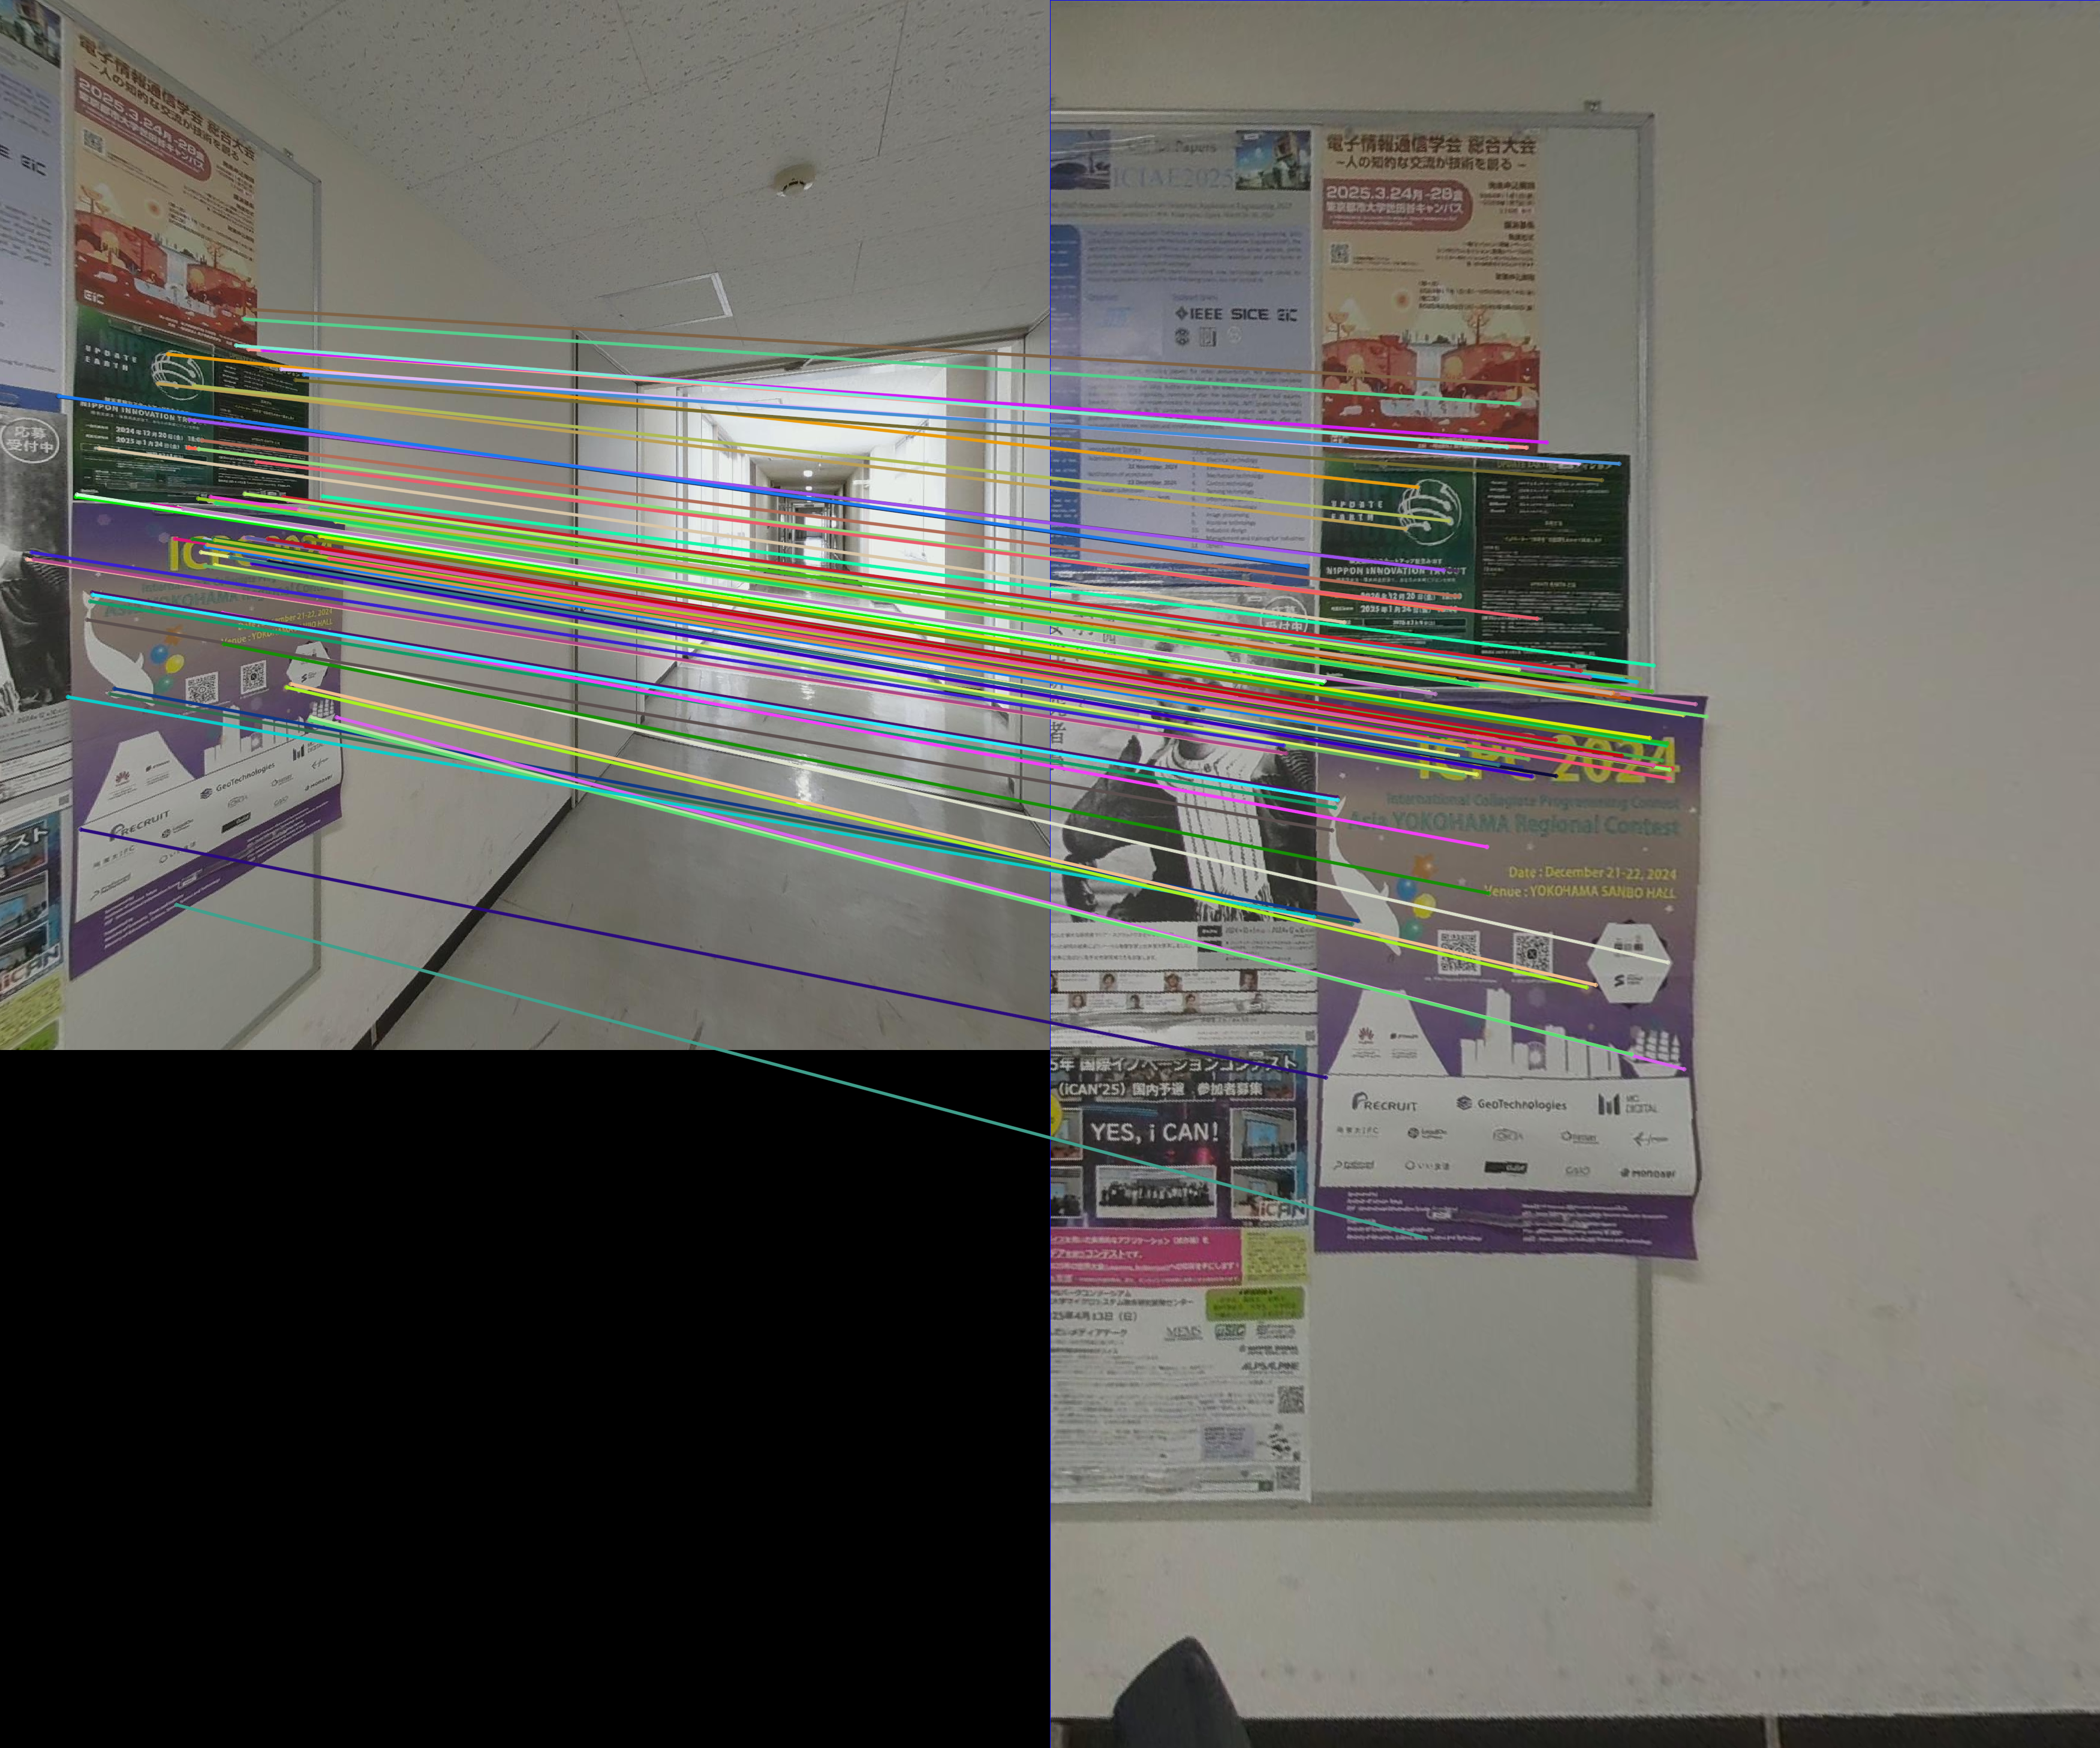
\includegraphics[width=0.7\textwidth]{figures/akaze.png}\\
    \end{tabular}
  \end{center}
  \caption{特徴点マッチング}
  \label{seven}
\end{figure}
ユーザの入力画像と3次元モデルのテクスチャ画像間で、多くの特徴点を正しく対応付けすることができている。

\subsection{自己位置推定の結果}
2次元-3次元特徴点の対応付け結果をもとに、自己位置推定を行い、
推定結果をもとに入力画像に3次元モデルのワイヤーフレームを描画した様子を図\ref{eight}に示す。
\begin{figure}[H]
  \begin{center}
    \begin{tabular}{c}
      \includegraphics[width=0.7\textwidth]{figures/result.png}\\
    \end{tabular}
  \end{center}
  \caption{自己位置推定の精度}
  \label{eight}
\end{figure}
実用上は問題ない程度の精度でモデルを描画することができている。
\section{今後の計画}
今後の研究計画を以下に示す。
\begin{enumerate}
  \item 3次元モデルの適用範囲の拡張
  \begin{itemize}
    \item より広範囲の空間を再現し、テクスチャ画像がさらに増えた場合も正しく類似画像を推定できるか調査
  \end{itemize}
  \item 全方位動画を活用したテクスチャ自動取得
  \begin{itemize}
    \item 静止画ではなく全方位動画を入力として用い、適切なフレームを自動で抽出することで、効率的なテクスチャ収集を実現
  \end{itemize}
  \item 自己位置推定機能を応用した実用的なアプリケーションの開発
  \begin{itemize}
    \item 生成された3次元モデルと自己位置推定を組み合わせ、目的地までのルートを提示するナビゲーションシステムを構築
  \end{itemize}
\end{enumerate}

最後に、\textbf{研究成果のバックアップは必ず取るようにしましょう。}少なくとも月に一回は。

%参考文献
\begin{thebibliography}{99}
  \bibitem{bib1}MarketsandMarkets,「Digital Twin Market Size, Share \& Industry Trends Growth Analysis Report」
  \bibitem{bib2}国土交通省 不動産・建設経済局 情報活用推進課,「屋内地図・屋内測位環境構築の手引き」6p
  \bibitem{bib3}菅谷保之,「直交射影の共線性と共面性を用いたカメラ姿勢の推定」
\end{thebibliography}

\end{document}
